\indent \section{Инженерная реализация модуля взаимодействия парсера русского языка с онтологией}

\subsection{Детали реализации}

Реализация предлагаемого решения производилась с использованием языка Haskell спецификации Haskell 2010 \cite{haskell2010}, добавляюшая в стандарт языка FFI, а также регламентирующей ряд синтаксических изменений. Для компиляции библиотеки использовался компилятор Glasgow Haskell Compiler (GHC) версии 7.4.2 под управлением XUbuntu Linux 12.10 (версия ядра 3.5.0, архитектура x86).

Для взаимодействия с парсером использовалось API Link Parser \cite{api}, для взаимодействия с онтологией были выбраны библиотеки hsparql, предоставляющая DSL для генерации SPRARQL-запросов, и rdf4h, описывающая типы данных RDF в нотации языка Haskell.

Для сетевого взаимодействия использовались методы, предоставляемые стандартной библиотекой GHC и Haskell Platform.

При разработке использовался текстовый редактор Sublime Text 2 и система управления версиями Git. Код библиотеки является открытым, распространяется свободно, и на момент написания диссертации был доступен по адресу \url{https://github.com/lumrandir/tomahawk}.

Для моделирования и описания демонстрационных онтологий использовалась система Protege.

Парсер был реализован в виде веб-приложения topor-web, поскольку это упрощало работу над пользовательским интерфейсом и позволяло обойти проблемы с демонстрацией под различными платформами.

\subsection{Руководство по развёртыванию и эксплуатации парсера русского языка Link Parser с библиотекой tomahawk}

\subsubsection{Предварительные замечания}

Для выполнения описанного в представленном руководстве процесса на компьютере пользователя должна быть установлена операционная система
Ubuntu (KUbuntu, XUbuntu, Linux Mint, Debian) либо иная операционная система, оснащённая пакетным менеджером apt. Рекомендуется использование Ubuntu 12.10.

Развёртывание парсера на компьютерах с другими Unix-системами с помощью данного руководства допустимо, однако, возможны отличия:
названия пакетов и используемые пакетные менеджеры и/или способы установки пакетов могут отличаться от представленных в руководстве, хотя
последовательность действий совпадает.

Развёртывание парсера на операционных системах Windows не является предметом рассмотрения данного руководства, поскольку связано с
дополнительными инфраструктурными сложностями, препятствующими достижению демонстрационной цели.

\subsubsection{Установка необходимых компонентов}

Поскольку topor-web представляет из себя веб-ориентированную
клиент-серверную систему, распространяющуюся в виде исходного кода, для
полноценного развёртывания нам понадобятся следующие компоненты:

\begin{list}{\labelitemi}{\leftmargin=1.5cm}
	\item nginx – проксирующий веб-сервер, задачей которого является
маршрутизация запросов из внешней сети в веб-приложение,
поддерживающее работу системы;
	\item redis – документ-ориентированное сетевое журналируемое хранилище
данных типа <<ключ-значение>>; используется в качестве кэширующего
хранилища возвращаемых из онтологии данных;
	\item ruby – интерпретатор языка программирования Ruby, с использованием
которого выполнена реализация веб-приложения;
	\item ghc – компилятор языка программирования Haskell, с использованием
которого выполнена реализация генератора запросов к онтологии tomahawk;
	\item gcc – компилятор языка программирования C, с использованием
которого реализовано ядро парсера Link Grammar;
	\item git – распределённая система контроля версий; использование этого
компонента опционально, получить исходный код можно в виде архива.
\end{list}

\subsubsection{Получение исходного кода системы}

Система topor-web распространяется в виде исходного кода. Это значит,
что пользователь системы должен самостоятельно собрать готовую систему.

Получить исходный код системы можно двумя способами:
\begin{list}{\labelitemi}{\leftmargin=1.5cm}
\item клонирование репозитария кода системы с помощью системы
контроля версий;
\item получение исходного кода в виде архива.
\end{list}

Для клонирования репозитария пользователь должен установить
систему контроля версий Git. В операционной системе Ubuntu установка Git
производится при помощи команды:

\begin{lstlisting}[language=bash]
sudo apt-get install git
\end{lstlisting}

После успешной установки системы Git пользователь должен перейти в
каталог, где будет располагаться система topor-web. Например, копия
репозитария может располагаться в домашней папке пользователя, переход в
котрую осуществляется командой:

\begin{lstlisting}[language=bash]
cd ~
\end{lstlisting}

Войдя в нужную директорию, пользователь должен выполнить
следующую команду:

\begin{lstlisting}[language=bash]
git clone git://github.com/lumrandir/topor-web.git
\end{lstlisting}

В результате выполнения этой команды пользователь получит наиболее
актуальный исходный код системы topor-web, который будет помещён внутрь
директории topor-web по текущему пути. То есть, полный путь к каталогу с
системой будет выглядеть как ~/topor-web. Этот каталог в дальнейшем будем
называть корневым каталогом приложения.

Второй способ заключается в следующем:

\begin{list}{\labelitemi}{\leftmargin=1.5cm}
\item получить архив исходного кода системы по следующей ссылке:
\url{https://github.com/lumrandir/topor-web/archive/master.zip};
\item распаковать полученный архив в нужную директорию.
\end{list}

Получение исходного кода выполняется командами:

\begin{lstlisting}[language=bash]
cd ~ && wget https://github.com/lumrandir/\
topor-web/archive/master.zip
unzip master.zip && mv topor-web\{-master,\}
\end{lstlisting}

После чего в каталоге topor-web внутри текущего также будет
располагаться актуальный исходный код системы.

\subsubsection{Установка интерпретатора языка программирования Ruby}

Для работы системы предпочтительно использовать стандартный
интерпретатор CRuby версии равной или выше 1.9.1.

Работа системы topor-web на альтернативных интерпретаторах (JRuby,
Rubinius, REE) не тестировалась и не гарантируется.

Установка CRuby в Ubuntu выполняется следующим образом:

\begin{lstlisting}[language=bash]
sudo apt-get install ruby
\end{lstlisting}

Вместе с пакетом ruby будет установлен менеджер библиотек Ruby gem.
Для работы системы потребуется установить библиотеку bundler:

\begin{lstlisting}[language=bash]
sudo gem install bundler
\end{lstlisting}

Bundler осуществляет контроль зависимостей, при запуске системы он
проверяет наличие необходимых ruby-библиотек. После установки bundler необходимо войти в корневой каталог
приложения и выполнить установку необходимых библиотек: 

\begin{lstlisting}[language=bash]
bundle install.
\end{lstlisting}

Проверить запуск системы можно с помощью команды: 

\begin{lstlisting}[language=bash]
bundle exec unicorn
\end{lstlisting}

Данная команда запустит многопоточный веб-сервер unicorn. Работу
приложения можно проверить, запустив веб-браузер и перейдя по адресу
\url{http://localhost:8080/version}. Пользователь должен увидеть текущую версию
приложения и статус библиотек парсера (в данном случае статус будет
<<Библиотеки недоступны>>).

\subsubsection{Установка компиляторов библиотек парсера}

Для сборки библиотек Link Grammar парсера пользователю потребуются
компиляторы gcc и ghc, также система контроля версий subversion.
Последовательность команд для сборки библиотеки парсера следующая
(выполняется в корневом каталоге приложения):

\begin{lstlisting}[language=bash]
sudo apt-get install subversion
svn co http://svn.abisource.com/link-grammar/trunk
link-grammar
cd link-grammar
sudo apt-get install make gcc automake libtool ant
./autogen.sh
./configure
make
sudo make install
sudo ldconfig
\end{lstlisting}

Приведённая последовательность действий устанавливает пакеты make
(система автоматизированной компиляции), gcc (GNU Compiler Collection ---
компилятор языка Си), automake и libtool --- генераторы конфигурационных
файлов компиляции. После установки пакетов осуществляется конфигурация
(создание сценариев компиляции с учётом текущего состояния системы) и
собственно сборка парсера. Последние два шага устанавливают собранные
библиотеки в системные каталоги и осуществляют их регистрацию.

Следующий шаг --- сборка модуля взаимодействия с онтологией:

\begin{lstlisting}[language=bash]
cd ../tomahawk
sudo apt-get install ghc cabal-install
make
\end{lstlisting}

Эта последовательность действий устанавливает компилятор ghc
(Glasgow Haskell Compiler) и пакетный менеджер cabal (аналог rubygems для
инфраструктуры языка Haskell).

Выполнив описанные выше шаги, пользователь может вновь запустить
сервер системы командой bundle exec unicorn из корневой папки
приложения и перейти на страницу \url{http://localhost:8080/version} в веб-браузере.
В случае корректной сборки и установки библиотек их статус изменится на
<<Доступны>>.

\subsubsection{Установка хранилища Redis}

Установка redis в системе Ubuntu осуществляется командой:
\begin{lstlisting}[language=bash]
sudo apt-get install redis-server
\end{lstlisting}

После успешной установки redis необходимо сконфигурировать. Пример
содержания конфигурационного файла:
\begin{lstlisting}[language=bash]
daemonize yes
pidfile /var/log/redis.pid
port 6379
bind 127.0.0.1
timeout 0
\end{lstlisting}

В Ubuntu готовый конфигурационный файл уже имеется по пути
/etc/redis/redis.conf. Запуск сервера redis осуществляется при помощи
команды:
\begin{lstlisting}[language=bash]
redis-server /etc/redis/redis.conf
\end{lstlisting}

При этом может возникнуть ошибка недостаточных прав пользователя.
Для обхода этой ошибки необходимо либо запускать redis-server с
повышенными
правами
(sudo
redis-server
/etc/redis/redis.conf), либо изменить пути к pidfile и logfile в
конфигурационном файле, после чего вновь запустить сервер с текущими
привилегиями.

\subsubsection{Установка проксирующего сервера nginx}

Задача nginx --- служить промежуточным (проксирующим) веб-сервером
между
внешней
сетью
и
веб-сервером
unicorn,
поддерживающим
функционирование системы topor-web.

Nginx так же требуется сконфигурировать, указав upstream-связь через локальный Unix-сокет с веб-сервером Unicorn. Файл конфигурации
располагается по пути /etc/nginx/nginx.conf, там же можно найти примеры конфигурации.

После
конфигурации
необходимо
запустить
сервер
nginx
с
повышенными привилегиями (sudo nginx).

Nginx будет <<слушать>> подключения на 80-м порту, соответственно,
пользователь должен предварительно открыть этот порт во внешнюю сеть. Эту
операцию можно выполнить с помощью следующей команды:
\begin{lstlisting}[language=bash]
sudo iptables -i INPUT -p tcp --dport 80 --j ACCEPT
\end{lstlisting}

\subsubsection{Работа с системой}

На этом этапе развёртывание приложения завершено. Чтобы проверить
его работу, необходимо в веб-бразуере компьютера, имеющего прямой сетевой
доступ к компьютеру, на котором развёртывалась система, перейти по адресу
http://<hostname>, где вместо <hostname> подставить ip-адрес или имя хоста
компьютера, на котором развёрнута система.

Рабочий сервер должен ответить html-страницей с формой следующего
вида (рисунок \ref{fig:form}).

\begin{figure}[H]
	\centering
		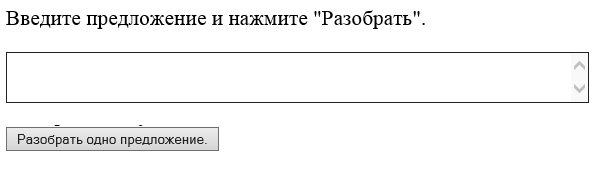
\includegraphics[scale=1.0]{images/form.png}
	\caption{\small Форма ввода системы topor-web}
	\label{fig:form}
\end{figure} 

Введите предложение в текстовое поле и нажмите кнопку <<Разобрать>>.
Пример разбора показан на рисунке \ref{fig:parse}.

\begin{figure}[H]
	\centering
		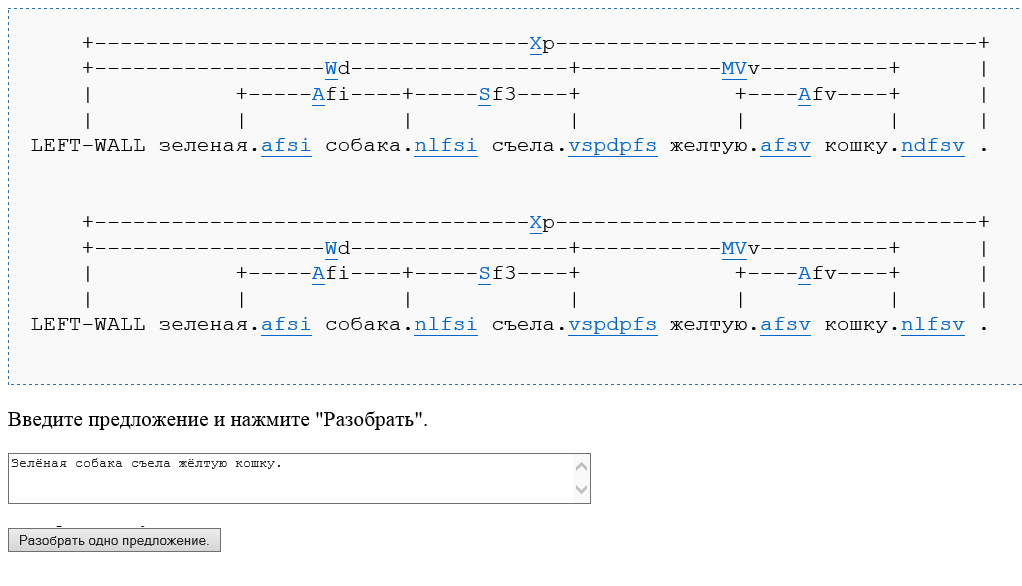
\includegraphics[scale=0.5]{images/parse.png}
	\caption{\small Пример разбора}
	\label{fig:parse}
\end{figure} 

Структура, представленная над полем ввода на рисунке \ref{fig:parse} является
деревом синтаксического разбора. Синий подчёркнутый текст – применяемые
к элементам предложения правила из онтологии.

\subsection{Результаты и выводы по главе 4}

В процессе работы над главой 4 были достигнуты следующие результаты:
\begin{list}{\labelitemi}{\leftmargin=1.5cm}
	\item рассмотрены детали инженерной реализации модуля взаимодействия парсера и онтологий tomahawk;
	\item составлено руководство по установке, настройки и работе с демонстрационной версией технологии topor-web.
\end{list}

\textbf{Вывод}: инженерная реализация спроектированного модуля выполнена успешно, полученной в процессе реализации информации достаточно для проведения экономического обоснования целесообразности внедрения предлагаемого решения.